\section{Wireless Telemetry Data} \label{section:WirelessTelemetryResearch}

The initial component to this project is the retrieval of wireless telemetry data. Telemetry is the automatic measurement and wireless transmission of data from a remote or inaccessible source for monitoring. The telemetry data source for this project is an 802.11ax Wi-Fi router acting as a Wireless Access Point. 

\subsection{ASUS ROG Rapture GT-AX11000 Router}

The ASUS ROG GT-AX11000 (provided by InterDigital) is a Tri-band 10 Gigabit Wi-Fi router with a quad-core CPU. It supports 2.4GHz, 5GHz-1 and 5GHz-2 bands with a combination of OFDMA and MU-MIMO technology to provide greater network capacity and efficiency. The use of Orthogonal Frequency Division Multiple Access (OFDMA) allows for one channel to transmit data to several devices at the same time (more on this later) \cite{OFDMA}. 

\subsection{ASUS Web GUI}

Out the box, ASUS provides an intuitive web Graphical User Interface (The ROG Gaming Centre) that acts as the main hub for total network control, with need-to-know information such as connected device status, server ping values, real-time network traffic and much more. Built into the web GUI are a multitude of features and operational settings, some of which will now be further explored. 

\subsubsection{Dash Board}

The Dash Board, as shown in Figure \ref{fig_ASUSwebGUI}, allows the network administrator to monitor real-time traffic metrics for the networking environment and analyse the real-time network ping and ping deviation.


\begin{figure} [ht]
    \centering
    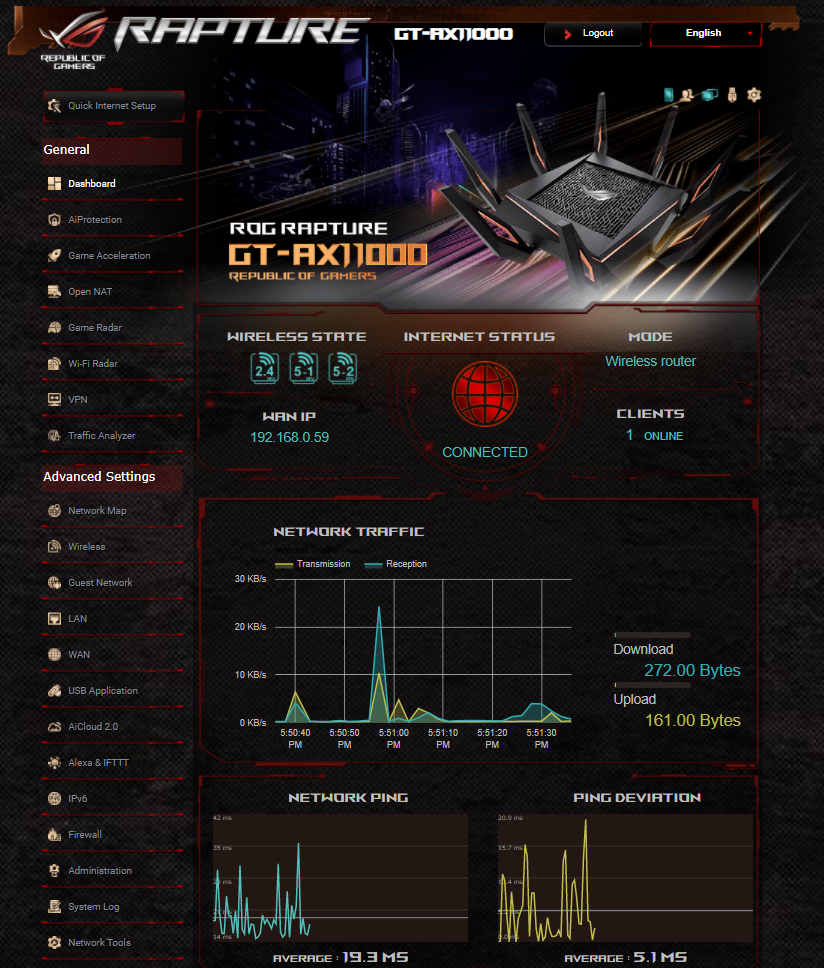
\includegraphics[width=1\linewidth]{pages/Chapter2/Chapter 2 images/ASUSwebGUI.PNG}
    \caption{ASUS ROG Gaming Centre.}
    \label{fig_ASUSwebGUI}
\end{figure}

\subsubsection{WiFi Radar}

WiFi Radar is an advanced analysis tool for the wireless network, it delves deep into the wireless channels and packet data intended for the purposes of troubleshooting. This feature permits the user to perform a Wi-Fi site survey in order to gather information on all nearby wireless access points. The site survey displays the signal strength, signal-to-noise ration (SNR), maximum physical rate, bandwidth and channel information. 




\begin{figure} [ht]
    \centering
    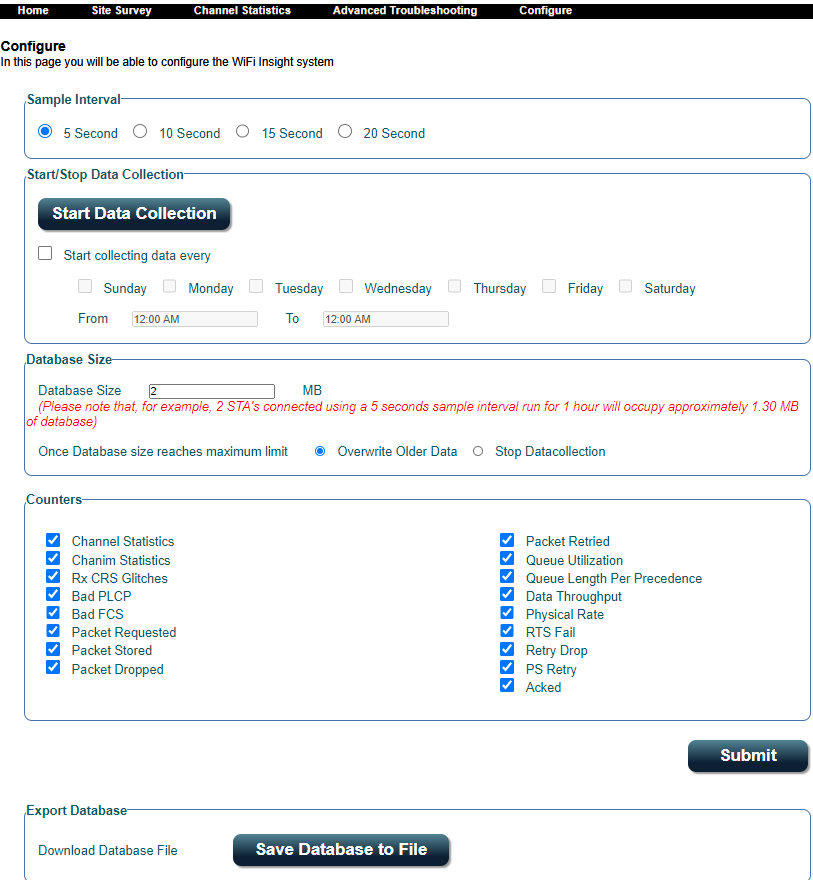
\includegraphics[width=1\linewidth]{pages/Chapter2/Chapter 2 images/WiFiRadarSetting.PNG}
    \caption{Advanced Troubleshooting Page on ASUS Web GUI.}
    \label{fig_WiFiRadar}
\end{figure}

Additionally, the Advanced Troubleshooting feature provides a telemetry data collection option, as shown in figure \ref{fig_WiFiRadar}, which produces a database with all technical data about the various advanced Wi-Fi parameters. This WiFi Radar component records data and generates a .DB file which is size configurable. This means that the user can define a maximum size that the database can reach after which it will either overwrite the older data or just stop data collection altogether. Also, the sample interval is configurable with settings to have data recorded every 5, 10, 15 or 20 seconds. Moreover, ASUS state that collecting data using a 5 second sample interval and with 2 STA’s (Stations) for 1 hour will approximately occupy 1.3MB of database, with new datasets being appended to the existing file. 

Appendix B Section \ref{ASUSEmail} shows an email correspondence with the ASUS customer service team asking to provide additional documentation for purposes of research and project work. Since ASUS could not provide additional information on what each parameter specifically measures and what the definition is for each one, research had to be conducted to fully understand what data could be extracted from the router.

Defined below are the wireless network parameters that can be recorded using the ASUS GT-AX11000 Wi-Fi router. 

\textbf{Channel Statistics}: Measures specific congestion metrics for each channel. A channel is a smaller subdivision of the WiFi frequency band through which wireless networks can send and receive data.

\textbf{Chanim Statistics}: Measure of channel interference.

\textbf{Rx CRS Glitches}: CRS (Certificate Signing Request) is a block of encoded text sent from an applicant to a Certificate Authority when applying for an SSL Certificate. It typically contains the public key for which the certificate should be issued, identifying information (such as a legal organisation name, domain name, locality and email address used to contact organisation) and integrity protection. A private key is also created at the same time as the CRS making a key pair \cite{CRS}. 

\textbf{Bad PLCP}: The PLCP (Physical Layer Convergence Protocol) maps the MAC protocol data units into a suitable frame format so they are ready for transmission by the Physical Medium Dependent. One of the other main operations of the PLCP is to route the incoming frames from the client to the MAC layer \cite{PLCP}. Bad PLCP is a receiver error metric \cite{PLCPPaper}. 

\textbf{Bad FCS}: FCS (Frame Check Sequence) is an error-detecting code added to a frame (frames are used to send payload data) \cite{FCS}. Bad FCS is the number of incoming packets where a Frame Error is detected. 

\textbf{Packet Requested/Stored/Dropped/Retired}: Count of number of packets requested, stored, dropped and retired per timestamp. 

\textbf{Queue Utilization}: A queue in networking is where packets of data ready to be forwarded are buffered before scheduling. The packets of data once in the queue are forwarded directly to the ingress (in) or egress (out) interfaces \cite{QOSPolicies}. In Queueing Theory, the Utilization factor is the amount of time that the system is busy. 

\textbf{Queue Length Per Precedence}: How many packets are transmitted between the AP and each connection, with certain packets given a priority. This is determined by the network scheduler (or packet scheduler) which manages the sequence of packets in the receive and transmit queues \cite{varghese_2005}. 

\textbf{Data Throughput}: How much data was transferred from a source at any given time (how many packets arrive at their destinations successfully). 

\textbf{Physical Rate}: The data rate obtained when data is actively transmitted. 

\textbf{RTS Fail}: When one node wants to transmit data to another node, it sends out a RTS (Request to Send) packet. The receiver node replies with a packet called CTS (Cleared to Send). After the transmitter node receives the CTS packet, it transmits the data packets. RTS Fail is the number of RTS packets sent without receiving a CTS packet response \cite{Karn1990MACAaNC}. 

\textbf{Retry Drop}: The number of attempts the wireless system makes to send a packet again before dropping the packet \cite{RetryDrop}. 

\textbf{PS  Retry}: The number of times packets are re-sent due to packet loss.  

\textbf{Acked}: Acknowledgement (ACK) is a signal that is sent by a device to show that data has been successfully transmitted, it is part of the communications protocol \cite{ackSignal}.


